documentclass[10pt,a4paper]{article}
\usepackage[utf8]{inputenc}
\usepackage{amsmath}
\usepackage{amsfonts}
\usepackage{hyperref}
\usepackage{graphicx}
\usepackage{amssymb}
\title{
		%\vspace{-1in} 	
		\usefont{OT1}{bch}{b}{n}
		\normalfont \normalsize \textsc{} \\ [25pt]
		\horrule \\[0.4cm]
		\huge Advanced Problem Solving(APS) \\Project Report \\ \\
	\\ \\
	    	\includegraphics[scale=1]{Music/mono.png} 
		\\ Submitted by:- \\ \\
		Anjul Ravi Gupta – 2018201021\\
	\\Kishan Shankar Singhal – 2018201023 \\ \\
	M. Tech CSE (2018-20)
		\horrule \\[0.5cm]
		\date{\vspace{-5ex}}
}
%\author{Kishan S Singhal}
\begin{document}
%\chapter*{Advanced Problem Solving(APS) \\             Project Report \\ }
\maketitle
%\part*{Advanced Problem Solving(APS) \\             Project Report \\ }

%\section*{Advanced Problem Solving (APS)\\\\Project Progress Report\\\\}
   
\section*{•Project Title}

      Binomial heap with applications (Implementation of Binomial heap on Kruskal’s or Prim’s Algorithm) and compare wrt AVL and Red-Black Tree.
      
%\section*{•Team Members}
%	Anjul Ravi Gupta – 2018201021\\
	%\\Kishan Shankar Singhal – 2018201023
\section*{•Project Objective}
	
	1. Implement the binomial heap and performed its comparative analysis with AVL and Red-Black trees on following standard operations:-\\
    • Insert\\
    • Delete\\
    • Search\\
\\To test the implementation using automated test cases with running time comparison on various input sizes (Graphical Analysis).\\

	2.Implement the Prim’s Algorithm using binomial heap and give its comparative analysis with standard Prim’s Algorithm (Priority Queue).\\ \\ 
	
\section*{•Technologies to be used}

	C/C++\\
	\\Latex\\
	\\Plotly(for graphical analysis)\\
	\\matplotlib


\section*{•Deliverables}

Our project contains the following files:\\
a) Program files\\
	(Seperate CPP files for Binomial heap, AVL, RB tree, Standard Prims and Prims using Binomial heap)\\

b) Input files \\
	(Files of varied input sizes, contain random, sorted ascending and sorted descending  numbers)\\
	
c) Report file \\
	(Containing all the detailed analysis of Binomial Heap with its application And time complexity)

	

\section*{•Binomial Heap} 

\subsection*{Introduction}
	A Binomial Heap is a collection of Binomial Trees.\\ \\
Binomial Tree:- \\
A Binomial Tree of order 0 has 1 node. A Binomial Tree of order k can be constructed by taking two binomial trees of order k-1 and making one as leftmost child or other.
A Binomial Tree of order k has following properties.
a) It has exactly 2k nodes.
b) It has depth as k.
c) There are exactly kCi nodes at depth i for i = 0, 1, . . . , k.
d) The root has degree k and children of root are themselves Binomial Trees with order k-1, k-2,.. 0 from left to right.\\ 

Binomial Heap:\\ \\
A Binomial Heap is a set of Binomial Trees where each Binomial Tree follows Min Heap property. And there can be at most one Binomial Tree of any degree. \\ \\


\subsection*{Implementation of Binomial Heap}

We have implemented the following functions for binomial heap:- \\ 
	

1. Union of Heaps:-\\
	struct node* unionofheaps (struct node* H1, struct node* H2) 
	
	In this function we are using the two functions below, to actually do union of two heaps  and returning binomial heap satisfying the binomial heap property.\\

1.1. Simply Merging:- 
	\\struct node* simplymerging(struct node* H1, struct node* H2) 
	
	In this function we are just merging the two heaps and returning new heap in ascending order of degrees of binomial trees in it.\\
	
	
1.2. Linking same degree nodes:-
	\\void linkingsamedegnodes(struct node* y, struct node* z) 
	
	In this function we are merging the two binomial trees of same degree n, into a binomial trees of n+1 degree.\\
	
2. Extract Minimum value node
	\\struct node* extractminnode(struct node* H)
	
	This function returns the minimum value node present in binomial heap.
	This function uses another function RevertingList which links the child nodes of the node removed and then union with the remaining heap. \\
	
3. Decrease Key
	\\int decreasekey(struct node* H, int i, int k) 
	This function changes the value of specified node i to the new value k. And reshuffle heap to maintain binomial heap property by moving the nodes to their respective correct positions.\\

	
4. Insertion
	\\Simply inserting values into binomial heap using union of heap function.\\
	
5. Deletion
	\\It uses the two functions i.e. Decrese key and extract min respectively to remove the node from the constructed binomial heap.\\
	
6. Search
	\\It simply searches the specified value in binomial heap.\\

\subsection*{Time Complexity Analysis}

\begin{tabular}{ |p{3cm}||p{6cm}||p{3cm}|  }
 \hline
 \multicolumn{3}{|c|}{Complexity Analysis of Binomial Heap} \\
 \hline
  Operation& Description & Complexity\\
 \hline
Insert & Inserts a new value  & O(log n)\\
Extract Minimum& Removes and returns the minimum value given a reference to the node & O(log n)   \\
Decrease key& Decreases an existing key to some value  &O(log n)\\
Union of heaps & Combine the heap with another to form a valid binomial heap  &O(log n)\\
Delete & Deletes a node given a reference to the node & O(log n)\\
 \hline
\end{tabular}


	\section*{•Testing} 
	
	We tested our implementation using automated test cases with running time comparison.
	For this we created input files for each of these operations:\\
	Insert, Delete and Search. \\ 

First, we have inserted 100 random elements, then 1000, and so on. 
Also we have done the same for deletion and search on all data structures used.\\

Similarly, we have performed the 3 operations on sorted data input file and reverse sorted data input file by taking different input sizes to measure insertion, search and deletion time. 
		
	Then, we have plotted the running time vs input size graph for all operations on all three data structures.\\


\section*{\\•Comparison of binomial heap with AVL and RB Tree}

\subsection*{Observations}

1. Insertion:- \\ \\
	In binomial heap, insertion takes lesser time than AVL and RB tree because the binomial heap consist of binomial tree and each binomial tree itself is a min heap and min heap insertion takes on an average lesser time than AVL and RB tree.\\ \\
	
2. Search:- \\ \\
	In binomial heap, search takes more time than AVL and RB tree since AVL and RB tree are binary search trees and hence value can be searched either on left or right subtree at each node. While in binomial heap, we have to search more nodes as values are not in sorted manner. \\ \\

3. Deletion:- \\ \\
	In binomial heap, deletion takes more time than AVL and RB tree since AVL and RB tree are binary search trees and hence value can be searched and deleted either on left or right subtree at each node. While in binomial heap, we have to search more nodes as values are not in sorted manner and then delete it. \\ \\
	
\subsection*{On Random Data set:}

\subsubsection*{1. Insertion}

Following graph shows the time comparison of inserting various input sizes on all the 3 data structures:-
	

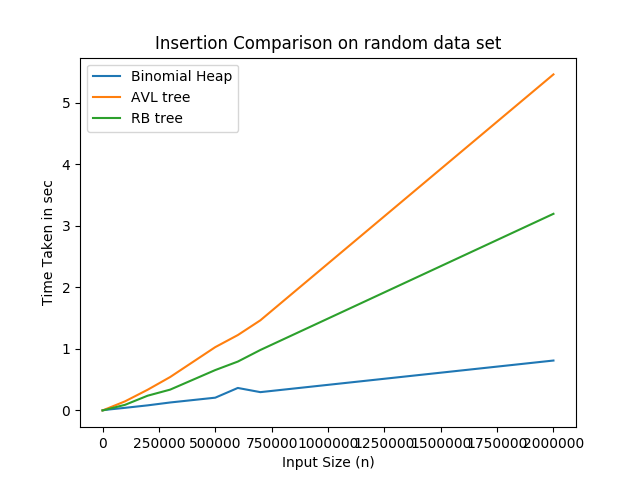
\includegraphics[scale=1]{insert.png} 


\subsubsection*{2. Searching}

Following graph shows the time comparison of searching various input values on all the 3 data structures:-\\ \\ \\ \\ 


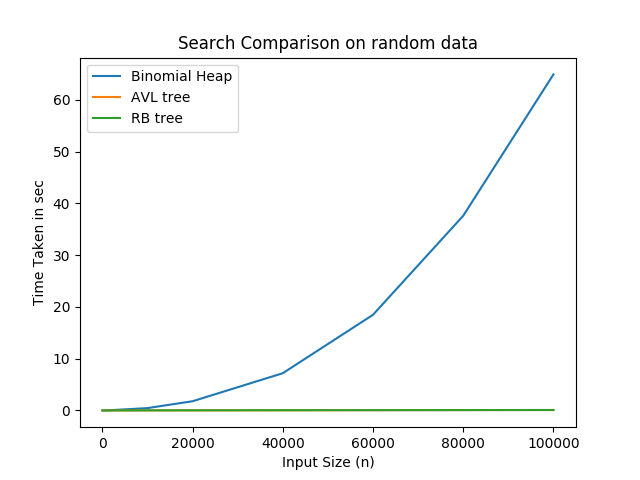
\includegraphics[scale=1]{s1.png}  \\ 


\subsubsection*{\\ \\ \\ \\ \\ \\ \\ 3. Deletion}

Following graph shows the time comparison of deleting various input sizes on all the 3 data structures:-


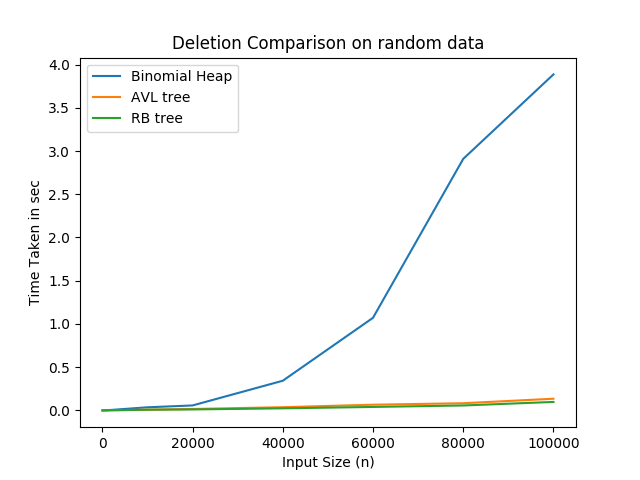
\includegraphics[scale=1]{delrr.png} 



\subsection*{On Sorted Data set:}

\subsubsection*{1. Insertion}

Following graph shows the time comparison of inserting various input sizes on all the 3 data structures:-
 

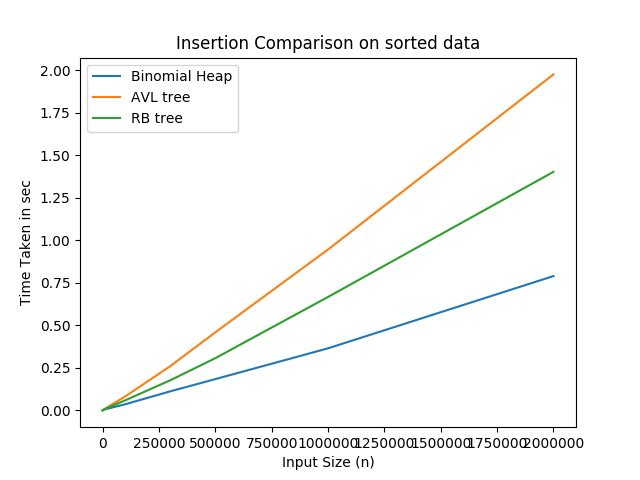
\includegraphics[scale=1]{sortedinsert.png}  

\subsubsection*{2. Searching}

Following graph shows the time comparison of searching various input values on all the 3 data structures:-


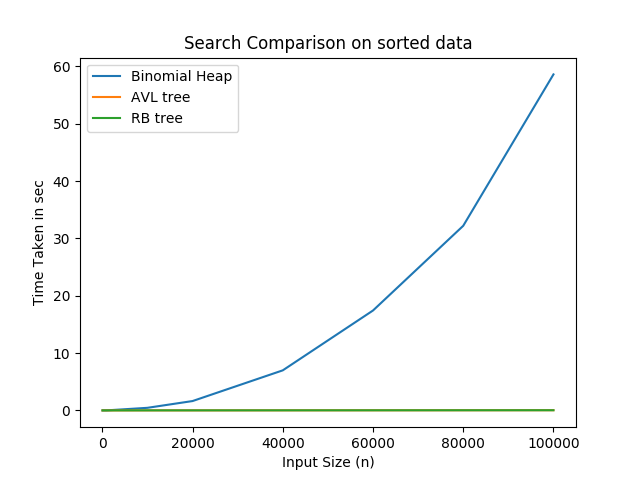
\includegraphics[scale=1]{sortii.png}  

\subsubsection*{3. Deletion}

Following graph shows the time comparison of deleting various input sizes on all the 3 data structures:-


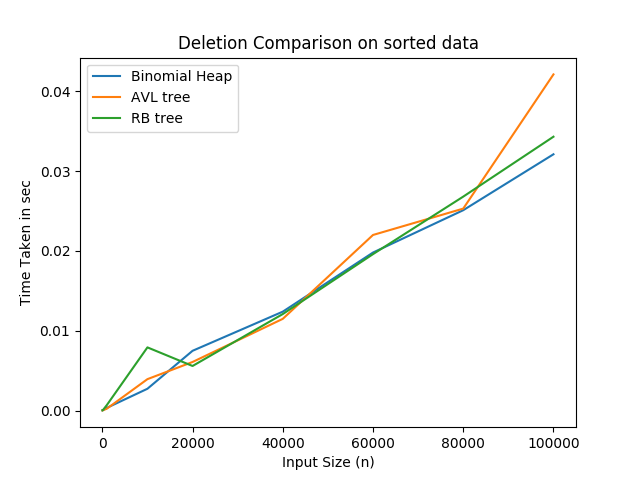
\includegraphics[scale=1]{ddss.png} 

\subsection*{On Reverse Sorted Data set:}

\subsubsection*{1. Insertion}

Following graph shows the time comparison of inserting various input sizes on all the 3 data structures:-
 

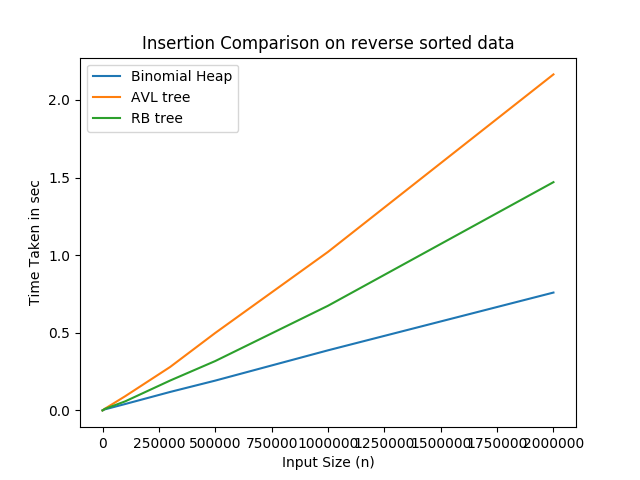
\includegraphics[scale=1]{reverseinsert.png}  

\subsubsection*{2. Searching}

Following graph shows the time comparison of searching various input values on all the 3 data structures:-


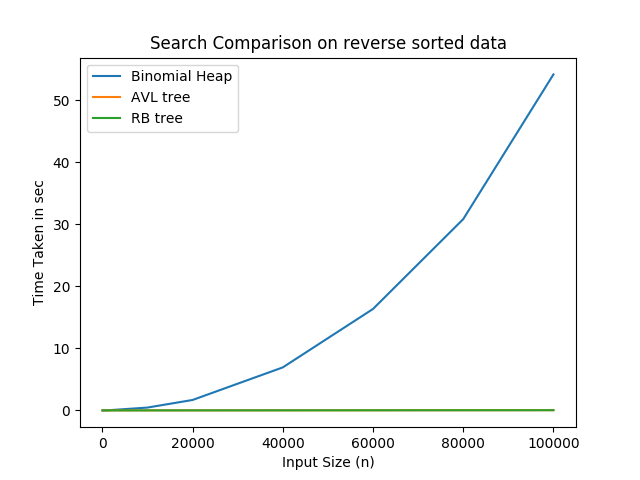
\includegraphics[scale=1]{rsooo.png}  

\subsubsection*{3. Deletion}

Following graph shows the time comparison of deleting various input sizes on all the 3 data structures:-


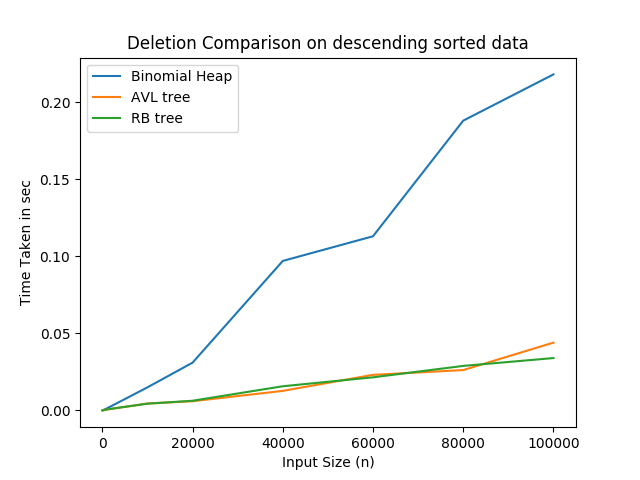
\includegraphics[scale=1]{dddd.png} 


\section*{•Application of Binomial Heap \\ Prim's Algorithm for MST} \\
	Prim's algorithm is a minimum spanning tree algorithm that takes a graph as input and finds the subset of the edges of that graph which form a tree that includes every vertex
has the minimum sum of weights among all the trees that can be formed from the graph.\\ \\

\subsection*{How Prim's algorithm works:-}\\ \\ 
	It falls under a class of algorithms called greedy algorithms which find the local optimum in the hopes of finding a global optimum.

	We start from one vertex and keep adding edges with the lowest weight until we we reach our goal. \\

The steps for implementing Prim's algorithm are as follows:\\ \\

1. Initialize the minimum spanning tree with a vertex chosen at random.\\
2. Find all the edges that connect the tree to new vertices, find the minimum and add it to the tree.\\
3. Keep repeating step 2 until we get a minimum spanning tree.\\

\subsection*{Standard implementation of Prims}
	Standard implementation of Prims uses the priority queue data structure.
	
\subsection*{Implementation of Prims using Binomial Heap}
	We have implemented the Prim's Algorithm using Binomial heap.\\ \\
	1. It uses Extract min function of binomial heap to select the edge with minimum weight  adjacent to the visited node and insert it into MST. \\ \\
	2. It uses Decrease key function is used to update the weight of nodes not yet included in the tree. As a result, a node that was thought to be too far may now move closer get extract min sooner. \\ \\
	
	
\subsection*{Comparison of Implementation of Prims using Binomial Heap and Priority queue}

The Prims implementation using binomial heap is taking lesser time as compared to standard priority queue implementation as it is using only two functions that are extract min and decrese key which takes much lesser time than priority queue. (Although both takes O(log n) to insert, remove). \\ \\

Following is small graph for time comparison:-


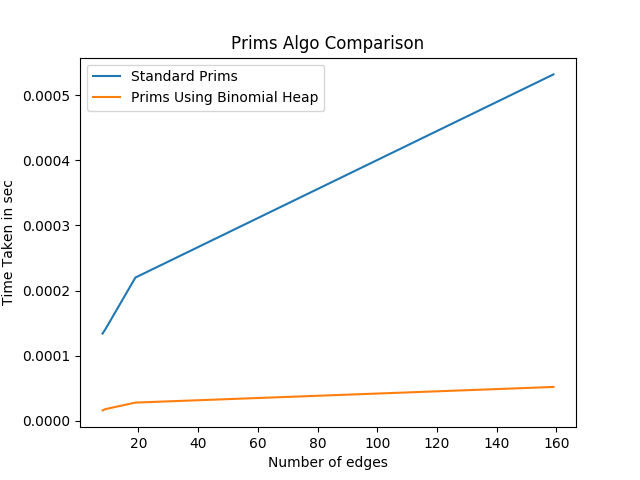
\includegraphics[scale=1]{prim.png} 

   \section*{•End user documentation} 


	Perform the following steps to run the program files:- \\ \\
1. \\Go to project directory and run \\
g++ binomialheap.cpp command through terminal.\\
The corresponding a.out will be generated. \\
Execute this file using the command ./a.out.\\
It will prompt for file name.\\ \\
Enter file name:- \\ \\
a) randomdata.txt for random input.(containing 2000000 numbers)\\
b) sortednumbers.txt for ascending sorted input.(containing 2000000 numbers)\\
c) reversesorted.txt for descending sorted input.(containing 2000000 numbers)\\ \\

Then, It will prompt for input size for insert, search, delete.\\
Enter size.\\

Then it will output the time for insertion, search and deletion for the given size data set.\\ \\
After that,
A menu will be prompted for the individual operation (if any) to be performed on a single element.\\
Like Insert, extract min, decrease key, print heap, etc.\\ \\ \\
	
2. \\Similarly, same above method can be used for time comparison for various operations on AVL and RB Tree.\\ 
Run g++ avltree.cpp for AVL on terminal inside project directory. Then ./a.out.\\ \\ 
Run g++ rbtree.cpp for AVL on terminal inside project directory. Then ./a.out.\\ \\ 
(These are also Menu Driven) \\ \\ \\

3. \\To run the application of binomial heap i.e. Prims algorithm, Do the below mentioned steps:- \\ \\a) Run g++ primbinomial.cpp on terminal inside project directory.\\
b) The corresponding a.out will be generated. \\
c) Also, Specify the testcase files made for different graphs on the command line argument on same line i.e. \\
d) Run the command\\ \\
./a.out graph1.txt\\
./a.out graph2.txt\\ etc,etc. \\

where graph1.txt.....graph2.txt etc are the sample test case files containing number of nodes, edges and weight of edges between any two vertices and act as input to our program. \\

e) It will output the weight of Minimal Spanning Tree (MST) along with the edges that are present in Minimal Spanning Tree (MST). \\ \\

4. \\To run the Standard Prims algorithm using priority queue, Do the below mentioned steps:- \\ \\a) Run g++ primPriorityQueue.cpp on terminal inside project directory.\\
b) The corresponding a.out will be generated. \\
c) It will prompt for number of vertices and edges. \\
d) Then for e number of edges, It will ask for start vertex, end vertex and their edge weight. \\
e) It will output the edges included in MST with weight of MST.\\ \\

5. Additionally, there are different .py files which are used to plot graphs for time analysis comparison for insert, search and delete.\\ \\
They can be run using command \\ \\
python (filename).py \\ \\

(It may prompt to error, then, install matplotlib using \\
pip install matplotlib \\
and run using above procedure). \\ \\

6. Also, we have provided number generation cpp files for random and sorted data. Running these files will generate test case file containing numbers which works as input to avl, rbtree and binomial heap programs. \\ \\ \\
		
		
		\section*{•Repository where work is being committed} \\ \\
		\url{https://github.com/AnjulGupta/APS\_project.git} \\ \\
		
		\section*{•References}
		\url{https://www.youtube.com/results?search_query=binomial+heap} \\ \\
     \url{https://www.growingwiththeweb.com/data-structures/binomial-heap/overview/} \\ \\
	\url{http://www.drdobbs.com/cpp/stls-red-black-trees/184410531} \\ \\
	\url{https://www.geeksforgeeks.org/} \\ \\
 
Books:- \\ \\
	Introduction-to-algorithms By Thomas H Cormen

	
	

\end{document}
